\documentclass[polish,envcountsect,10pt]{beamer}

    \usepackage[T1]{fontenc}
    \usepackage{polski}
    \usepackage{babel}

    \usetheme{EastLansing}

    \title{Pamięć masowa w Kubernetesie}
    \author{inż. Wojciech Baranowski \and inż. Michał Łubiński}
    \date{Gdańsk, 2024}

\begin{document}

\frame{\titlepage}

\begin{frame}{Ephemeral storage}
	Pamięć efemeryczna jest tymczasowa i związana bezpośrednio z instancją maszyny wirtualnej.
	\begin{itemize}
		\item Tymczasowość
		\item Wysoka wydajnosć
		\item Niski koszt utrzymania
	\end{itemize}
\end{frame}

\begin{frame}{Ephemeral storage}
	Przykładowe zastosowania:
	\begin{itemize}
    	\item Tymczasowe przechowywanie danych sesji w aplikacjach internetowych.
    	\item Pliki tymczasowe generowane podczas obliczeń i analizy danych.
    	\item Cache aplikacji, które mogą być łatwo odtworzone.
	\end{itemize}
\end{frame}

\begin{frame}{Persistent storage}
	Pamięć trwała jest zaprojektowana do długoterminowego przechowywania danych, niezależnie od stanu instancji maszyny wirtualnej.
	\begin{itemize}
		\item Trwałość
		\item Elastyczność
		\item Wyższy koszt
		\item Bezpieczeństwo
	\end{itemize}
\end{frame}

\begin{frame}{Persistent storage}
	Przykładowe zastosowania:
	\begin{itemize}
    	\item Bazy danych.
   		\item Systemy plików przechowujące dane użytkowników (np. zdjęcia, dokumenty).
    	\item Kopie zapasowe i archiwizacja danych.
	\end{itemize}
\end{frame}

\begin{frame}{PersistentVolume}
	PersistentVolume (PV) to zasób w klastrze Kubernetes, który reprezentuje rzeczywiste wolumeny dyskowe. PV jest niezależny od węzłów klastra.
	\begin{itemize}
		\item Trwałość
		\item Dostępność
		\item Różnorodność
		\item Poziomy dostępu (RWO, ROX, RWX)
	\end{itemize}
\end{frame}

\begin{frame}{PersistentVolume}
	\begin{figure}[H]
    	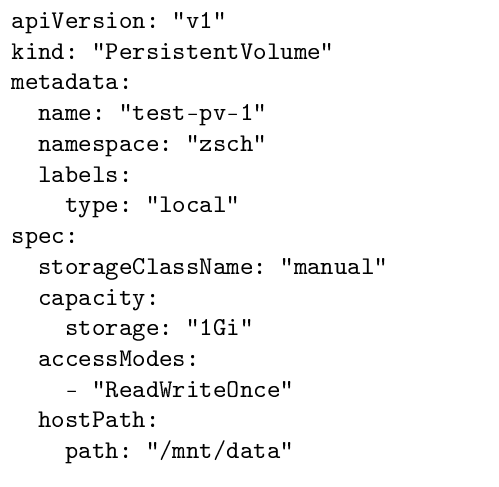
\includegraphics[width=0.5\linewidth]{images/pv.png}
	\end{figure}
\end{frame}

\begin{frame}{PersistentVolumeClaim}
	PersistentVolumeClaim (PVC) jest żądaniem zasobu PV przez aplikację w klastrze Kubernetes.
	\begin{itemize}
		\item Abstrakcja
		\item Dynamika działania
		\item Elastyczność
	\end{itemize}
\end{frame}

\begin{frame}{PersistentVolumeClaim}
	\begin{figure}[H]
    	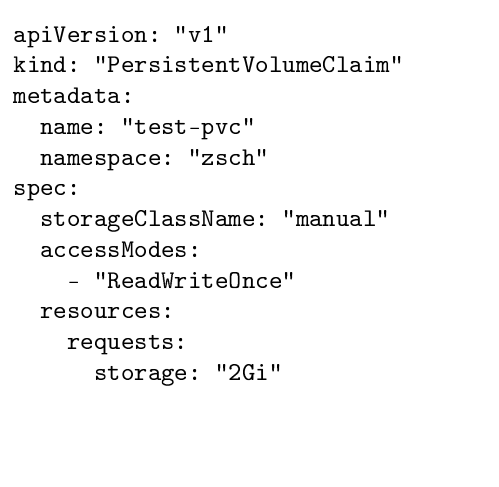
\includegraphics[width=0.5\linewidth]{images/pvc.png}
	\end{figure}
\end{frame}

\begin{frame}{StorageClass}
	Storage class jest zasobem używanym do automatycznego zarządzania i provisionowania zasobów typu storage w klastrze. Storage class umożliwia zdefiniowanie różnych klas pamięci masowej, które mogą być wykorzystywane w zależności od potrzeb. StorageClass zawiera następujące atrybuty:
	\begin{itemize}
		\item Provisioner
		\item Parameters
		\item ReclaimPolicy (Retain, Recycle, Delete)
		\item BindingMode (Immediate, WaitForFirstConsumer)
	\end{itemize}
\end{frame}

\begin{frame}{StorageClass}
	\begin{figure}[H]
    	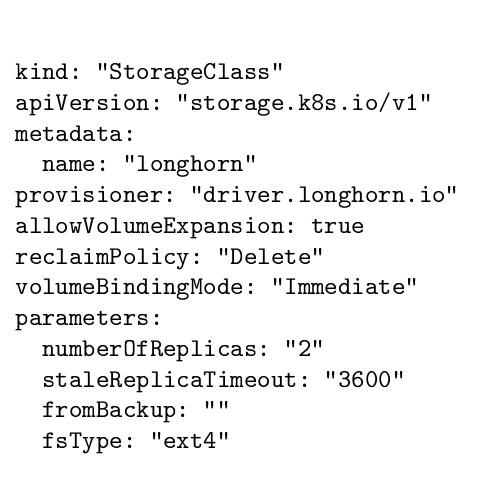
\includegraphics[width=0.5\linewidth]{images/sc.png}
	\end{figure}
\end{frame}

\begin{frame}{Storage blokowy}
	Storage blokowy odnosi się do przechowywania danych w postaci bloków. Każdy blok jest niezależnie adresowany i może być przechowywany w róćnych miejscach. Zastosowania:
	\begin{itemize}
		\item Przechowywanie danych dla baz danych i systemów wysokiej wydajności
		\item Idealny dla aplikacji o dużej intensywności I/O
		\item Podstawowy storage w przypadku VM
	\end{itemize}
\end{frame}

\begin{frame}{Storage blokowy}
	Zalety:
	\begin{itemize}
		\item wysoka wydajność
		\item elastyczność
		\item bezpieczeństwo
	\end{itemize}
	\medskip
	Wady:
	\begin{itemize}
		\item złożoność zarządzania
		\item koszty
	\end{itemize}
\end{frame}

\begin{frame}{Storage plikowy}
	Storage plikowy przechowuje dane w postaci plików i katalogów, które są organizowane w strukturze hierarchicznej. Zastosowania:
    \begin{itemize}
		\item Aplikacje o mniejszej intensywności I/O
		\item Systemy współdzielenia plików oparte o sieć (NAS)
		\item Środowiska wymagjące zrównoleglonej pracy nad plikami
	\end{itemize}
\end{frame}

\begin{frame}{Storage plikowy}
	Zalety:
	\begin{itemize}
		\item Łatwość użycia
		\item Współdzielenie danych
		\item Koszty
	\end{itemize}
	\medskip
	Wady:
	\begin{itemize}
		\item Wydajność
		\item Skalowalność
		\item Ograniczenia systemów plików
	\end{itemize}
\end{frame}

\begin{frame}{Mechanizmy provisioningowe}
\end{frame}

\begin{frame}{Longhorn}
	\begin{figure}[H]
    	
\includegraphics[width=0.4\linewidth]{images/longhorn.png}
	\end{figure}
\end{frame}

\begin{frame}{Longhorn}
	Zalety:
	\begin{itemize}
		\item Pełna integracja z kubernetesem
		\item Łatwość konfiguracji przez UI oraz CLI
		\item Automatyczna replikacja danych
		\item Obsługa snapshotów i backupów
		\item Ławte skalowanie
	\end{itemize}
	\medskip
	Wady:
	\begin{itemize}
		\item Wymaga dodatkowych zasobów na replikowane dane
		\item Mniej wydajny, niż mechanizmy natywnie działające w przestrzeni jądra
	\end{itemize}
\end{frame}

\begin{frame}{GlusterFS}
	\begin{figure}[H]
    	
\includegraphics[width=0.4\linewidth]{images/glusterFS.png}
	\end{figure}
\end{frame}

\begin{frame}{GlusterFS}
	Zalety:
	\begin{itemize}
		\item Wysoka skalowalność 
		\item Automatyczna replikacja danych 
		\item Funkcje snapshotów 
	\end{itemize}
	\medskip
	Wady:
	\begin{itemize}
		\item Skomplikowana konfiguracja i zarządzania (CLI + heketi) 
		\item Wymaga manualnej konfiguracji
		\item Problemy wydajnościowe w dużych klastrach
	\end{itemize}
\end{frame}

\begin{frame}{Ceph RBD}
	\begin{figure}[H]
    	
\includegraphics[width=0.4\linewidth]{images/ceph.png}
	\end{figure}
\end{frame}

\begin{frame}{Ceph RBD}
	Zalety:
	\begin{itemize}
		\item Wysoka wydajność i skalowalność 
		\item Automatyczna replikacja i zarządzanie uszkodzonymi dyskami 
		\item Obsługa snapshotów i klonowania wolumenów 
	\end{itemize}
	\medskip
	Wady:
	\begin{itemize}
		\item Złożoność zarządzania 
		\item Wymaga zaawansowanej wiedzy technicznej 
		\item Wymaga dużych nakładów zasobów 
	\end{itemize}
\end{frame}

\begin{frame}{CephFS}
	\begin{figure}[H]
    	
\includegraphics[width=0.4\linewidth]{images/ceph.png}
	\end{figure}
\end{frame}

\begin{frame}{CephFS}
	Zalety:
	\begin{itemize}
		\item Wysoka skalowalność i elastyczność 
		\item Automatyczna replikacja i zarządzanie uszkodzonymi dyskami 
		\item Obsługa snapshotów i klonowania wolumenów 
	\end{itemize}
	\medskip
	Wady:
	\begin{itemize}
		\item Złożoność zarządzania 
		\item Wymaga zaawansowanej wiedzy technicznej 
		\item Wymaga dużych nakładów zasobów 
	\end{itemize}
\end{frame}

\begin{frame}{iSCSI}
	\begin{figure}[H]
    	
\includegraphics[width=0.4\linewidth]{images/iscsi.png}
	\end{figure}
\end{frame}

\begin{frame}{iSCSI}
	Zalety:
	\begin{itemize}
		\item Wysoka wydajność
		\item Szeroka kompatybilność i wsparcie 
	\end{itemize}
	\medskip
	Wady:
	\begin{itemize}
		\item Wymaga konfiguracji sieciowej i zarządzania siecią 
		\item Brak natywnej replikacji 
		\item Problemy w przypadku awarii sieci 
	\end{itemize}
\end{frame}

\begin{frame}{Porównanie}
	\begin{itemize}
		\item Klaster złożony z 3 węzłów master i 16 węzłów worker
		\item Baza danych SQLite z podmontowanym PVC
		\item RWO dla storage'u blokowego i RWX dla storage'u plikowego
		\item Operacje I/O na kolejno 1, 2, 4 i 8 wątkach
		\item Phoronix Test Suite
	\end{itemize}
\end{frame}

\begin{frame}{Porównanie}
	\begin{figure}[H]
    	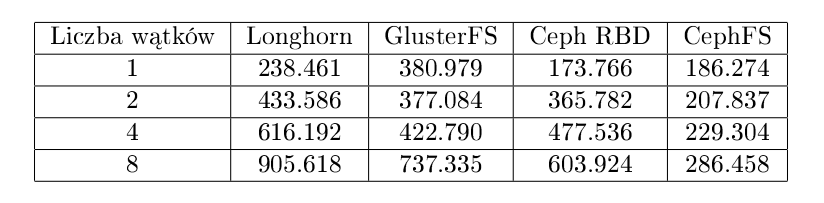
\includegraphics[width=0.9\linewidth]{images/table.png}
	\end{figure}
\end{frame}

\begin{frame}{GlusterFS - przykład z życia}
	Ile może zająć rebalance 250Gb danych?
	\begin{figure}[H]
    	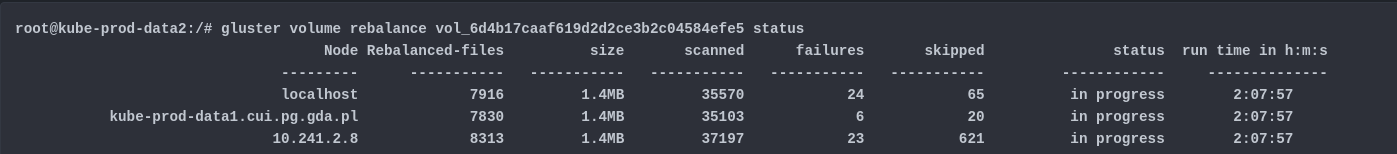
\includegraphics[width=\linewidth]{images/noeta.png}
	\end{figure}
\end{frame}

\begin{frame}{GlusterFS - przykład z życia}
	302 dni!
	\begin{figure}[H]
    	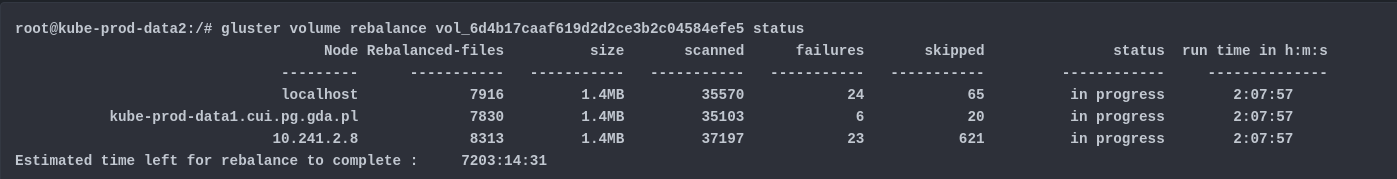
\includegraphics[width=\linewidth]{images/eta.png}
	\end{figure}
\end{frame}

\begin{frame}{GlusterFS - przykład z życia}
	Rozwiązanie:
	\begin{figure}[H]
    	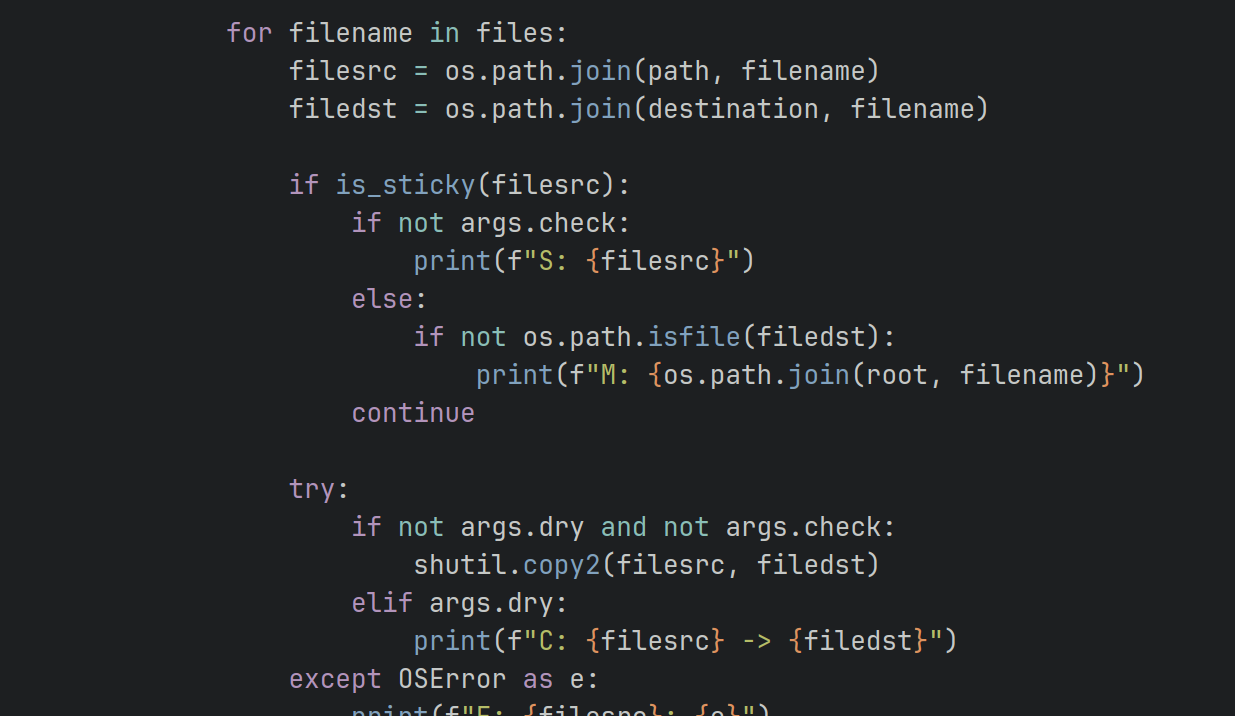
\includegraphics[width=\linewidth]{images/script.png}
	\end{figure}
\end{frame}

\begin{frame}{GlusterFS - przykład z życia}
	A co w przypadku storage'u blokowego?
\end{frame}

\begin{frame}{Pytania?}
\end{frame}

\begin{frame}{Źródła}
	\begin{itemize}
		\item slajdy wykładowe
		\item materiały udostępnione przez Centrum Usług Informatycznych PG
		\item skrypt udostępniony przez Kacpra Donata
		\item https://kubernetes.io/docs/home/
		\item https://longhorn.io
		\item https://www.gluster.org
		\item https://ceph.io
		\item https://en.wikipedia.org/wiki/ISCSI
		\item wiedza własna
	\end{itemize}
\end{frame}

\end{document}
